\chapter{Introduction}
\label{chapter:introduction}

\section{Overview of the work}

\subsection{Real world meterial approach}
\begin{itemize}
    \item Organics
    \begin{itemize}
      \item Skin (sweaty, dry, makeup)
      \item Fruits (layered, uniform, non-uniform)
      \item Food (Cheese, meat, bread)
    \end{itemize}
    \item Non-organic
    \begin{itemize}
      \item Marble (polished, rough, dusty)
      \item Plastics (wax, etc othe non-organic uniform solid bodies)
    \end{itemize}
    \item Liquids (milk, wine, juice, dirty/dusty water, ocean water)
    \item Fluids (air, fog, dust)
    \item Snow
    \item Thin sheets (paper, foilage, cloth)
    \item Non photoreal (Cartoon style and stylisation)
\end{itemize}

\subsection{Things to consiger while choosing method}
\begin{description}
  \item [Lighting restrictions] \emph{Analytic light} sources and \emph{area lights and IBL} friendly
  \item [Multiple object friendly]
  \item [Preprocess] Is additional preprocess step needed (point cloud generation)
  \item [Parametrization] Artist friendly or physically correct
  \item [Performance] Is it a real time approximation for OpenGL
  \item [Flickering] How suitable for animation (does it introduce additional flickering)
  \item [Motion blur] How well it works with motion blur (SSS and volumetrics)
  \item [Closed objecs only] Does it supports single sided geometry
  \item Homogeneous or inhomogeneous
  \item Istropic or anisoisotropic media
\end{description}

Focus on the rendering highly scattering materials with relatively small mean
free path length between scattering events.

Do not consider spectral scattering. Only monochromatic light is simulated.
There are papers describing the process of combined rendering of RGB with
corresponding importance sampling.

Why not to use point cloud based approach:
\begin{itemize}
    \item{Ease of use for the user. Don't want to introduce more parameters to
    control and require the end use to know the underlying algorithms}
    \item{Undesired preprocessing step. Unfriendly to progressive rendering}
    \item{Density of the generated PC limits the scope of the available
    parameters. It restrics the effective width of the SSS by minimal distanse
    between points. Point density $\approx$ mean free path}
    \item{Workflow complications for storing PC and additional memory
    requirements}
    \item{Possible flickering artifacts during animation}
    \item{Additional memory required}
\end{itemize}

\section{Unidirectional path tracing}
Unidirectional path tracing \gls{UDPT} or simply path tracing is one of the
fundamental methods of Monte Carlo light integration in computer graphics.

\ldots

A typical disadvantage of the classic \gls{UDPT} is the high variance and
subsecuently strong noise component in the rendered images of the scenes with 
highly non-uniform incoming illumination.
In practice, these scenes contain small but intensive emitters or direct sun
light in the image-based lighting scenes. The extreme worst case is the
prensence of the analytic light sources: point lights with zero area or
directional lights, having virtually infinite distance to the shaded locaten.

\subsection{UDPT with direct light sampling}
Although \gls{UDPT} is proved to be a robust unbiased estimator, it has some
limitations.
\begin{figure}
    \centering
    \begin{subfigure}{0.45\textwidth}
        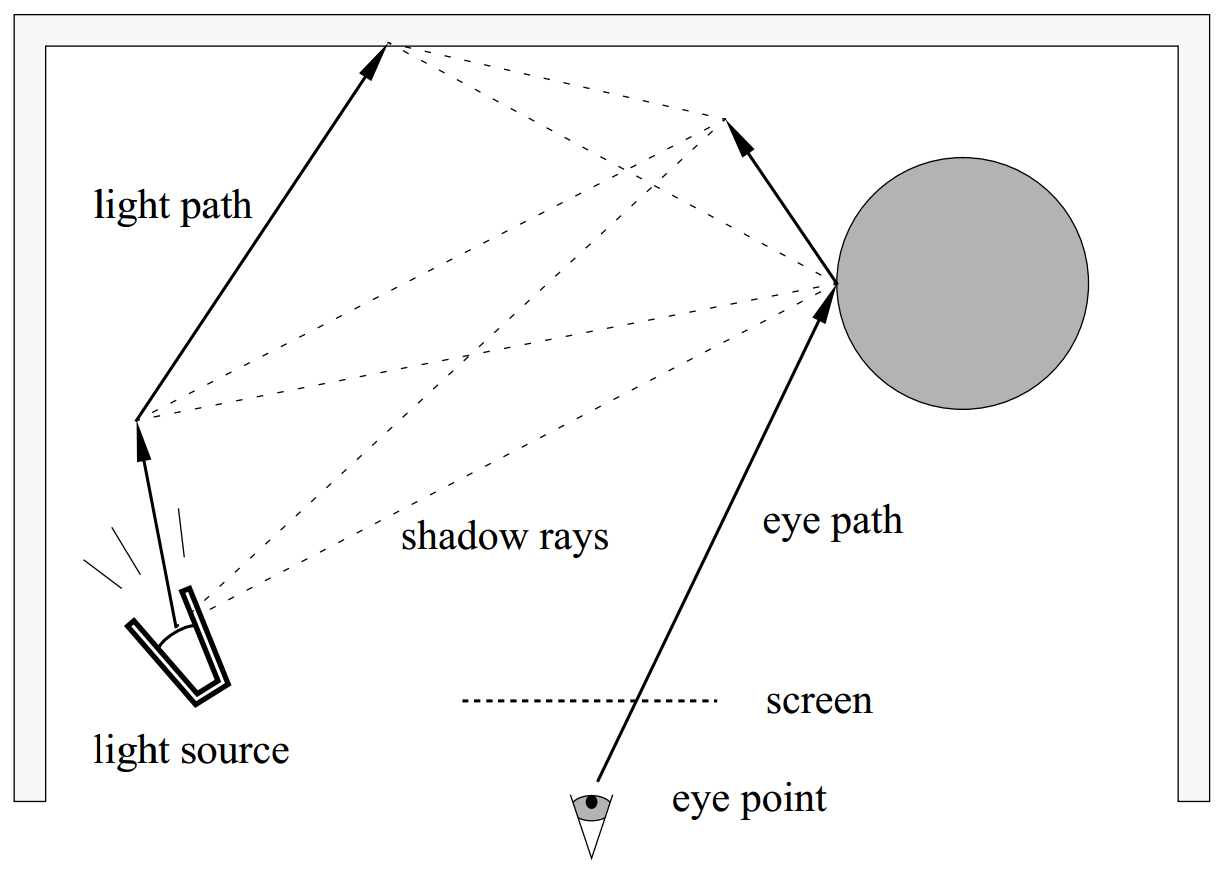
\includegraphics[width=\textwidth]{imgs/schemes/generalized_BDPT_lafortune}
        \caption{general}
        \label{fig:bdptgeneral}
    \end{subfigure}
    \quad
    \begin{subfigure}{0.45\textwidth}
        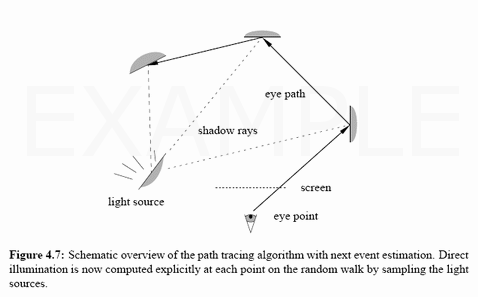
\includegraphics[width=\textwidth]{imgs/schemes/PT2_resize}
        \caption{special}
        \label{fig:udpt_ptdl}
    \end{subfigure}

    \caption{BDPT temp illustrations}
    \label{fig:bdpt}
\end{figure}


Next Event Estimation (\gls{NEE}) is one of the common methods of reducing a
variance of the path tracing. The main idea of the \gls{NEE} is to estimate
\textit{direct illumination} by sampling the light source directly at each step
of the path tracing. Then, the shadow test ray is needed to ensure that the
current light sampling position in visible by the surface.

\gls{NEE} can also be considered as the special case of the general
Bidirectional Path Tracing algorithm \gls{BDPT} \cite{Veach:94:BDPT}.
\ref{fig:bdpt} Using the vocabulary of the original paper, NEE algorithm is
\textit{(m,2)-method}. with the length of light path equals 2 and length of the eye path $m\geq3$ is defined by
the \gls{UDPT} settings.

\subsection{Volumetric Path Tracing}
Path tracing with light scattering inside the media
Dwivedi sampling scheme

\subsection{Volumetric path tracing with Next Event Estimation}
The idea of direct light sampling can be applied to the volumetric path tracing
as well.
The generalized theory of \gls{BDPT} in participating media was first described
by Lafortune ans Willems in \cite{Lafortune:1996:RPM:275458.275468}. 

\ldots

Preforming the direct light estimation from inside the media with the refractive
boundry proved to be a non-trivial task.
Due to the refraction on the boundary between materials with different index of
refraction (\gls{IOR}), the light from the emitter to the scattering point never
travels by a straight light. Except the casse of the normal incident rays. To
satisfy the Fermat's principle
\footnote{Fermat's principle or the principle of least time states that the path taken between two points by a ray of light is the path that can be traversed in the least time}
we have to construct the path with the middle point somewhere on the boundry.

To my knowledge, there are no robust and fast enough methods for solving this
complication in general way. Although, there are considerable iterative
approaches described in the literature during last years
\cite{holzschuch:hal-01083246}, \cite{10.1111:cgf.12681}, \cite{Koerner2016}.

In this work I have decided to consider the situation when the bounary
refraction can be neglected. In the other words, the materials with \gls{IOR}=1.
It leads to the approximation of the direct light path from inside the media to the light source as a straigt line. This assumption certainly
introduces an error in the simulation. But the error is significant only for
optically low dense materials. Light propagation in highly scattering media, in
contrast, is charachterized by many scattering events. Which makes the direction
of the first ray less important for the future light simulation.


